% Overleaf notes:
% 1. Please compile with XeLaTeX.
% 2. For strict ACL formatting, create a new project from the official ACL
%    template and replace its main .tex body with this file. The template
%    should provide acl.sty. If acl.sty is unavailable, upload it from the
%    official ACL template.
\documentclass[11pt]{article}
\usepackage[final]{acl}
\usepackage{times}
\usepackage{latexsym}
\usepackage{graphicx}
\usepackage{booktabs}
\usepackage{tabularx}
\usepackage{multirow}
\usepackage{url}
\usepackage{hyperref}
\usepackage{fontspec}
\usepackage{xeCJK}

\setmainfont{Times New Roman}
\IfFontExistsTF{Noto Serif CJK SC}{
  \setCJKmainfont{Noto Serif CJK SC}
}{
  \setCJKmainfont{FandolSong-Regular}
}
\IfFontExistsTF{Noto Sans CJK SC}{
  \setCJKsansfont{Noto Sans CJK SC}
}{
  \setCJKsansfont{FandolHei-Regular}
}

\title{面向 WebShop 的微调与策略控制结合的 LLM Agent}

\author{
  Group 34 \\
  CS40008.01 / LLM 2026 \\
  \texttt{https://github.com/yilinliao520-eng/group-34}
}

\begin{document}
\maketitle

\begin{abstract}
本文研究 WebShop 交互式购物环境中的大语言模型智能体。该任务要求模型理解自然语言购物目标，生成检索查询，比较商品页面，并在有限步数内完成购买决策。我们以 Qwen2.5-7B-Instruct 的 ReAct 智能体为基线，依次评估关键词检索提示、监督微调（SFT）、失败模式诊断和轻量级 anti-loop 策略控制器。实验显示，原始 ReAct 在 50 条 full synthetic goals 上的 strong success rate 为 10\%，关键词提示将其提升到 20\%。然而，直接使用统一轨迹训练得到的 SFT 模型反而下降到 2\%，主要原因是模型容易重复搜索而不进入点击或购买阶段。加入保守的 anti-loop 控制器后，统一 SFT 模型达到 48\% strong success rate，是本项目中表现最好的配置。结果表明，SFT 可以改善部分语言理解与检索行为，但 WebShop 这类交互式任务仍然需要显式的阶段转换控制。
\end{abstract}

\section{引言}

Web shopping 是一个具有现实意义的语言智能体任务：模型不仅要理解用户约束，还要将目标转化为可检索的关键词，浏览商品结果，选择具体商品和选项，并判断何时购买。与单轮问答不同，WebShop 要求智能体在多个动作之间保持状态一致性，因此它同时考验语言理解、检索、页面阅读和交互策略。

本项目最初采用三阶段思路：首先建立 ReAct baseline，然后通过 SFT 学习更好的行动轨迹，最后引入奖励感知的策略控制。实际实验中我们发现，朴素 SFT 并没有直接带来收益。进一步诊断表明，SFT 模型虽然能生成更像训练数据的查询，但经常陷入 repeated-search/no-buy loop，即反复搜索而不点击商品，或已经进入商品页面却不购买。因此，我们将实验重点转向失败模式分析，并实现了一个确定性的 anti-loop controller 作为轻量策略层。

本文贡献可以概括为三点：第一，在 full WebShop 商品索引上复现并比较 ReAct、关键词提示和 SFT 智能体；第二，通过失败诊断解释 SFT 失效的主要原因；第三，证明简单的阶段转换控制器可以显著改善 SFT 智能体的交互成功率。

\section{相关工作}

WebShop 是一个面向真实电商交互的 benchmark，包含大规模商品库、自然语言 shopping goals 和基于 reward 的评价方式 \cite{yao2022webshop}。ReAct 框架通过交替生成 reasoning 和 action，使语言模型能够在交互环境中逐步决策 \cite{yao2022react}。在偏好学习方面，DPO 将 preference optimization 转化为直接优化 chosen/rejected response 的目标函数 \cite{rafailov2023dpo}，理论上适合修正 WebShop 中的局部动作偏好，例如 repeated search 与 click 之间的选择。

与这些工作相比，本项目不是追求 benchmark-level SOTA，而是在课程项目范围内分析一个小型 LLM agent pipeline 的真实失败模式。我们的主要发现是：对于 WebShop，模型生成能力和交互控制能力不能简单等同。SFT 学到的局部语言模式如果没有合适的状态转换约束，可能会损害整体任务成功率。

\section{任务与数据}

我们使用 WebShop full mode，共包含约 1.18M 个商品，并构建完整 Lucene 检索索引。每个 episode 中，智能体接收一个购物目标，并通过文本动作与环境交互。主要动作包括 \texttt{search[keywords]}、\texttt{click[ASIN]}、\texttt{click[option]} 和 \texttt{click[Buy Now]}。

主实验使用 synthetic goals 0--49，共 50 条任务，每个 episode 最多 7 步。我们报告两个指标：平均 reward 和 strong success rate。Strong success 定义为 episode reward 大于 0.5。需要强调的是，该设置用于课程项目中的受控比较，并不是原始 WebShop benchmark 的完整 500-goal 测试。

\section{方法}

\subsection{ReAct Baseline}

原始 baseline 使用 Qwen2.5-7B-Instruct，根据当前 observation 生成一个简短 thought 和一个 WebShop action。该方法的优点是结构简单、可解释性较好；主要缺点是模型常生成过长、过自然语言化的搜索查询，导致检索结果质量不稳定。

\subsection{关键词检索提示}

早期实验显示，search query 的质量对 WebShop 成败影响很大。原始 ReAct 往往把完整购物目标直接塞进 \texttt{search[]}，包含大量修饰语和约束条件。我们加入 keyword-only prompt，要求模型在搜索阶段使用 3--6 个关键词，优先保留商品类型、品牌、尺寸、颜色、功能等高信息量词。该修改不改变模型参数，只改变查询生成行为。

\subsection{监督微调}

我们使用 LoRA adapter 对模型进行 SFT，训练数据来自清洗后的 WebShop-style trajectories 和 query examples。SFT 的目标是让模型学习更稳定的搜索和行动格式。实验中我们分别尝试专家轨迹与统一清洗轨迹，其中 unified SFT 是后续诊断和 controller ablation 的主要对象。

\subsection{失败诊断}

SFT 后的 aggregate performance 明显下降，因此我们没有继续盲目扩大训练，而是对 episode 进行失败类型统计。主要失败包括 zero-result search、repeated search、max-step no-buy、wrong product 和 premature buy。其中最突出的现象是 repeated-search/no-buy loop：模型在应该点击商品时继续搜索，或在商品页附近没有及时购买。

\subsection{Anti-loop Controller}

基于诊断结果，我们实现了一个确定性的 anti-loop controller。它不是学习得到的 Bandit，而是一个策略控制原型，核心规则包括：

\begin{itemize}
    \item 如果模型重复生成相同或高度相似的搜索动作，则强制点击当前可见商品；
    \item 如果连续搜索次数过多，则从搜索阶段转入点击阶段；
    \item 如果已在商品页面且接近最大步数，则保守触发购买动作。
\end{itemize}

该控制器的目标不是替代语言模型，而是修正 SFT 在交互阶段转换上的系统性错误。

\subsection{DPO 准备}

DPO 是本项目后续自然延伸，尤其适合构造 action-level preference pairs，例如 ``重复搜索'' 作为 rejected action，``点击候选商品'' 作为 chosen action。然而，当前最终正向结果不依赖 DPO。我们只保留了 DPO 数据构造计划和训练脚本，没有将 DPO 结果作为已完成贡献报告。

\section{实验结果}

\begin{figure}[t]
    \centering
    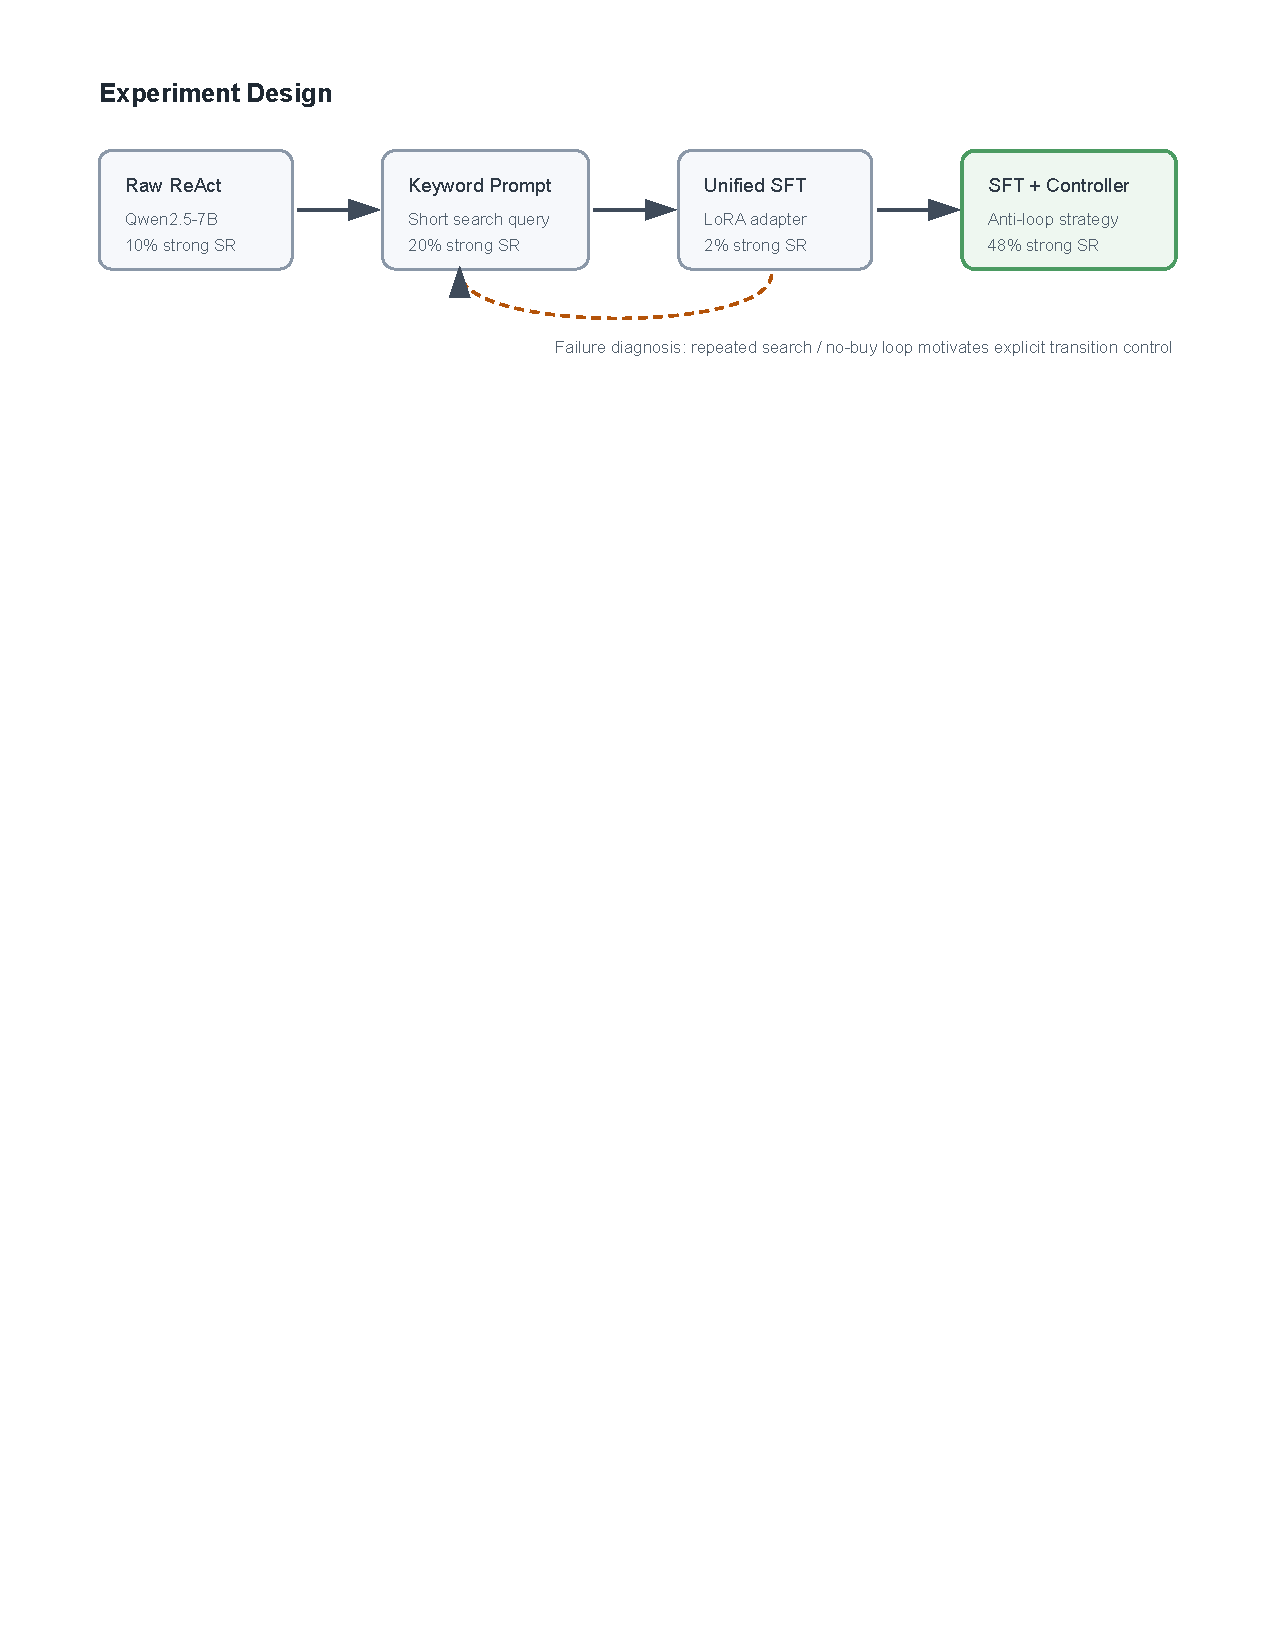
\includegraphics[width=\linewidth]{figures/workflow.pdf}
    \caption{实验流程。从原始 ReAct 出发，依次加入关键词提示、SFT、失败诊断和 anti-loop controller。诊断发现 SFT 的主要问题是 repeated-search/no-buy loop，因此最终采用 SFT 与策略控制结合的结构。}
    \label{fig:workflow}
\end{figure}

\begin{table}[t]
\centering
\small
\begin{tabularx}{\linewidth}{lrrX}
\toprule
系统 & Strong SR & Avg. Reward & 说明 \\
\midrule
Raw ReAct & 10\% & 0.077 & 原始 ReAct 提示 \\
Keyword baseline & 20\% & 0.209 & 短关键词搜索提示 \\
Unified SFT & 2\% & 0.012 & 反复搜索，几乎不购买 \\
Unified SFT + conservative controller & 48\% & 0.419 & 当前最佳配置 \\
\bottomrule
\end{tabularx}
\caption{50 条 full synthetic goals 上的主实验结果。}
\label{tab:main}
\end{table}

表 \ref{tab:main} 展示了主实验结果。Raw ReAct 的 strong success rate 为 10\%，说明原始模型在 WebShop 中具备一定零样本交互能力，但稳定性较弱。关键词提示将 strong success rate 提升到 20\%，验证了 query reformulation 对检索任务的重要性。Unified SFT 单独使用时只有 2\%，说明模仿轨迹格式并不等于学会完整交互策略。加入 conservative controller 后，strong success rate 提升到 48\%，平均 reward 达到 0.419。

\begin{figure}[t]
    \centering
    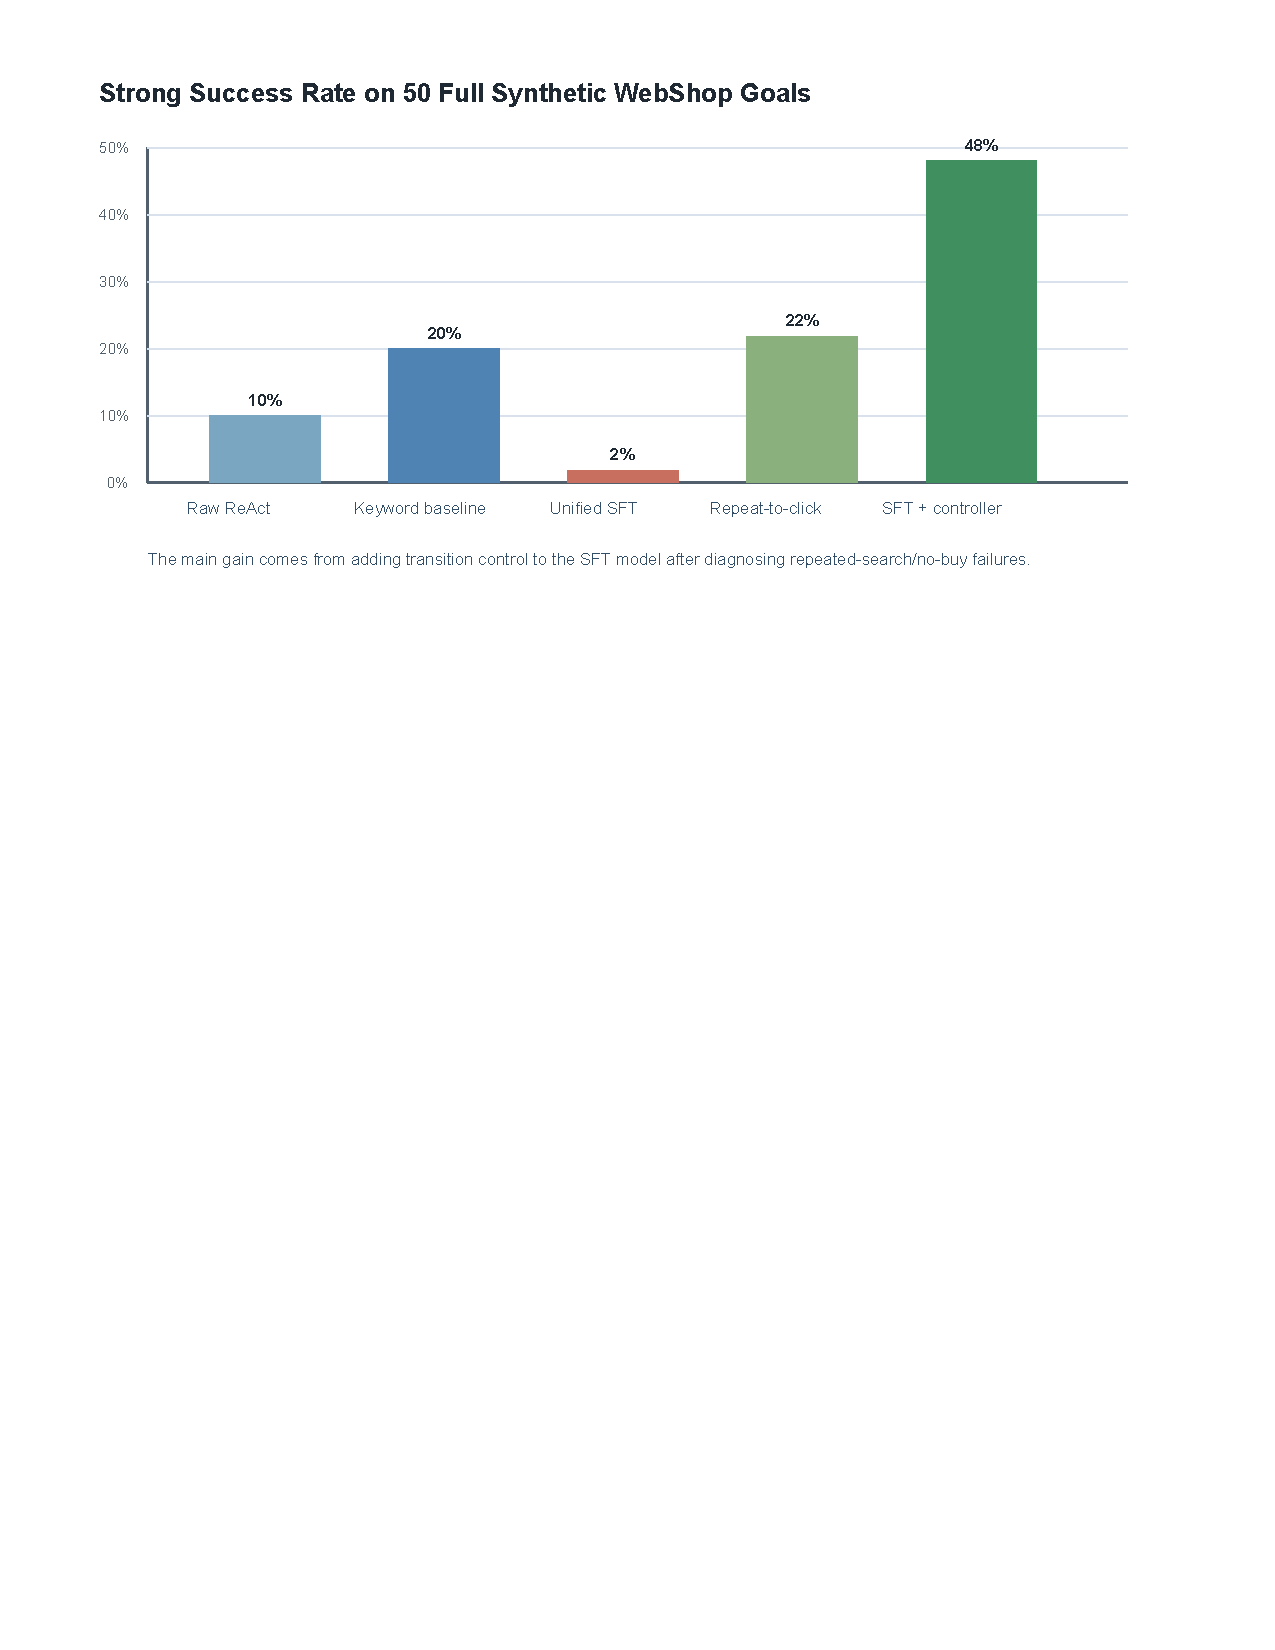
\includegraphics[width=\linewidth]{figures/main_results.pdf}
    \caption{主要系统的 strong success rate 对比。SFT 单独使用明显失效，而加入阶段转换控制后取得最高成功率。}
    \label{fig:main-results}
\end{figure}

\begin{table}[t]
\centering
\small
\begin{tabularx}{\linewidth}{lrr}
\toprule
Controller 变体 & Strong SR & Avg. Reward \\
\midrule
No controller & 2\% & 0.012 \\
Repeat-to-click only & 22\% & 0.182 \\
No forced buy & 22\% & 0.192 \\
Conservative forced buy & 48\% & 0.419 \\
Aggressive controller & 48\% & 0.446 \\
\bottomrule
\end{tabularx}
\caption{Unified SFT 上的 controller ablation。}
\label{tab:ablation}
\end{table}

表 \ref{tab:ablation} 进一步说明 controller 的有效成分。仅加入 repeat-to-click 规则即可从 2\% 提升到 22\%，说明搜索到点击的阶段转换是关键瓶颈。若不允许 forced buy，成功率仍停留在 22\%。加入保守购买规则后，成功率达到 48\%。Aggressive controller 的平均 reward 略高，但 strong success rate 与 conservative controller 相同；考虑到误买风险，本文将 conservative controller 作为主结果。

\section{分析与讨论}

实验结果表明，WebShop agent 的难点不只是生成正确文本动作，还包括在合适时间从一个阶段转入下一个阶段。关键词提示之所以有效，是因为它直接改善了检索入口；SFT 之所以失败，是因为它学习到了局部动作形式，却没有稳定学习 ``搜索--点击--选择--购买'' 的全局流程。

这一现象也解释了为什么 controller 可以带来较大提升。Controller 不需要理解所有商品细节，它只负责在明显循环或接近步数上限时强制推进状态。因此，语言模型和策略控制器形成了互补：模型负责理解目标和生成候选动作，controller 负责限制无效循环并保持任务进度。

从实验设计角度看，本文最重要的经验是：当 SFT 结果异常下降时，不能只通过增加训练轮数或扩大数据继续尝试，而应先检查真实 episode 的失败模式。否则，模型可能在 aggregate metric 上持续退化，而研究者无法判断问题来自检索、动作格式、购买时机还是奖励定义。

\section{局限与未来工作}

本项目仍有明显局限。首先，主实验只在 50 条 synthetic goals 上评估，结论不能直接等同于完整 WebShop benchmark。其次，controller 是确定性规则，不是学习得到的 Bandit，因此只能视为策略控制原型。第三，DPO 尚未形成可靠的训练和评估闭环；尤其是 preference pair 必须严格对齐同一 observation 下的 chosen/rejected action，否则会引入噪声甚至错误学习信号。

未来工作可以沿三条方向推进：第一，扩大评估到更多 synthetic goals 或 human goals；第二，构造 observation-aligned DPO 数据，专门修正 repeated search、no-buy 和 premature buy；第三，将当前规则 controller 替换为 contextual Bandit 或轻量 learned policy，使策略层能够根据 observation、检索结果数量和历史动作自适应决策。

\section{结论}

本文围绕 WebShop 构建并分析了一个 Qwen2.5-7B-Instruct 智能体实验链路。实验显示，原始 ReAct 可以完成少量任务，关键词提示能改善检索表现，但朴素 SFT 会因 repeated-search/no-buy loop 显著退化。通过失败诊断引入 conservative anti-loop controller 后，统一 SFT 模型在 50 条 full synthetic goals 上达到 48\% strong success rate。该结果说明，在交互式购物任务中，微调语言模型需要与显式策略控制结合，才能更稳定地完成多步决策。

\begin{thebibliography}{9}

\bibitem{yao2022webshop}
Shunyu Yao, Howard Chen, John Yang, and Karthik Narasimhan.
\newblock 2022.
\newblock WebShop: Towards Scalable Real-World Web Interaction with Grounded Language Agents.
\newblock In \textit{Advances in Neural Information Processing Systems}.

\bibitem{yao2022react}
Shunyu Yao, Jeffrey Zhao, Dian Yu, Nan Du, Izhak Shafran, Karthik Narasimhan, and Yuan Cao.
\newblock 2023.
\newblock ReAct: Synergizing Reasoning and Acting in Language Models.
\newblock In \textit{International Conference on Learning Representations}.

\bibitem{rafailov2023dpo}
Rafael Rafailov, Archit Sharma, Eric Mitchell, Stefano Ermon, Christopher D. Manning, and Chelsea Finn.
\newblock 2023.
\newblock Direct Preference Optimization: Your Language Model is Secretly a Reward Model.
\newblock In \textit{Advances in Neural Information Processing Systems}.

\end{thebibliography}

\end{document}
